\subsection{Track Requirements}\label{subsec:track-requirements}

HelixRM's Requirement Tracking feature is essential for keeping
track of the software needs of any project.
It helps to maintain requirements clear, connected to
deliverables, and tracked against their fulfilment criteria.

With a defined plan for managing the requirements,which
are essential to maintaining the project's high quality and
making sure it satisfies the expectations of the stakeholders,
such an organised approach improves project management.

\paragraph{Why Track Requirements} Serve as clear descriptions of a specific software product\cite{j_e__archer_2003}
and as more precise measurements for when a need is met\cite{evangelos_markopoulos__2009}.


\paragraph{Advantages of Monitoring Requirements}
Using user-centered design concepts, enhances personalisation to satisfy requirements\cite{maria_grazia_violante__2017}.
It also provides a structure for examining how needs have changed over time, for well-informed decision-making\cite{evangelos_markopoulos__2009}.

\paragraph{Real World Usage}
Tracking requirements is used in multiple software projects, in order to monitor and address criteria in order to produce higher-quality results\cite{edward_r__rang__1985}.
It is also used in product lifetime management, making it easier to include requirement management into more comprehensive processes for the product lifetime\cite{maria_grazia_violante__2017}.

Even while it might be very advantageous, it might be
argued that the extra difficulty of managing all those needs
could just result in increased costs and possibly create project
timeline delays.
For most people, striking a balance between meticulous
tracking and nimble approaches is never easy.

With HelixRM, tracking requirements is made easier, offering a
comprehensive interface for managing requirements,
ensuring that all elements are traceable and manageable with the use of categories like:
\begin{itemize}
    \item Tag: a unique identifier for the requirement
    \item Summary: a brief description of the requirement
    \item Type: Functional, Non-functional, \ldots
    \item Importance: High, Medium, Low/ MoSCoW / \ldots
    \item Status: Draft, In Review, Approved, Rejected, \ldots
\end{itemize}

\begin{figure}[htbp]
    \centerline{
        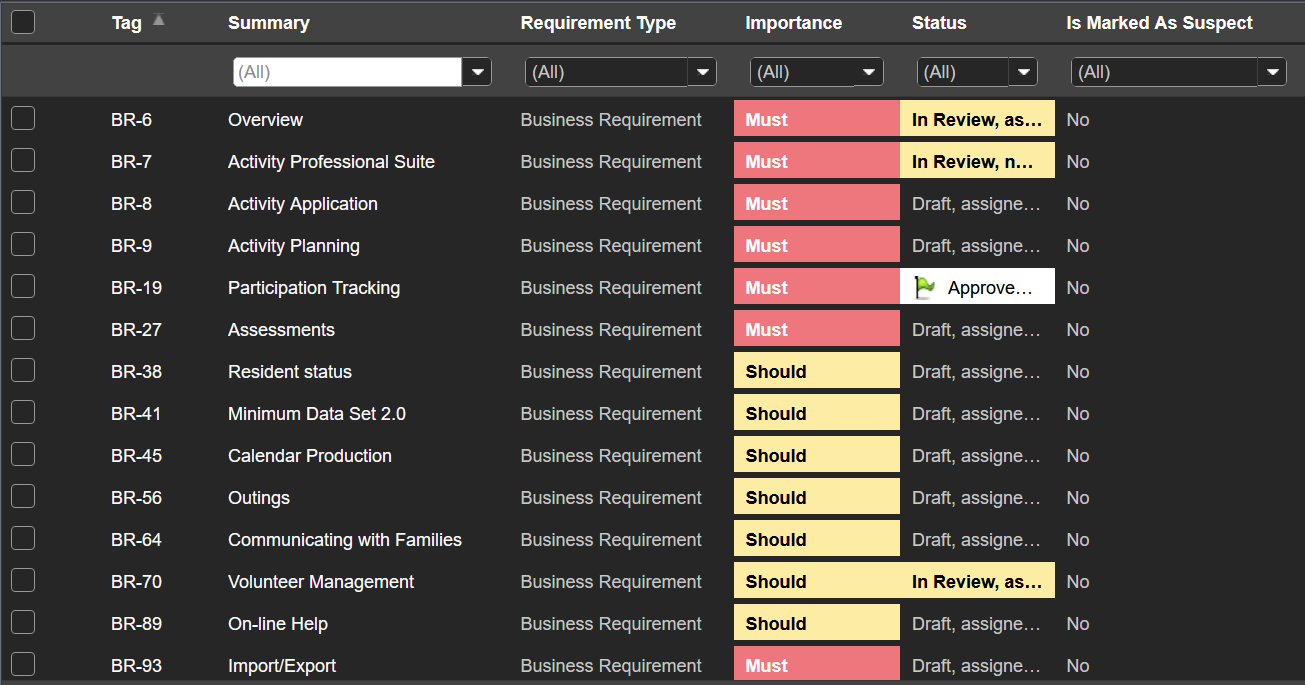
\includegraphics[width=\linewidth]
        {images/requirement-tracking}
    }
    \caption{HelixRM requirement tracking interface.}
    \label{fig:fig}
\end{figure}


